\documentclass{beamer}
\usetheme{Madrid}
\usecolortheme{default}

\usepackage{amsmath}
\usepackage{amssymb}
\usepackage{booktabs}
\usepackage{graphicx}
\usepackage{algorithmic}
\usepackage{tikz}
\usepackage{xcolor}
\usetikzlibrary{positioning, shapes.geometric, arrows.meta, calc, decorations.pathreplacing}

\title[GEC Progress]{Global Expert Choice Networks:\\Progress Update}
\author{Hanchi Sun}
\institute{Lehigh University}
\date{\today}

\begin{document}

\frame{\titlepage}


%%%%%%%%%%% Feb 18 progress update %%%%%%%%%%%

\begin{frame}{Feb 18, 2026: Progress Update (GEC)}
\begin{itemize}
    \item \textbf{Paper:} Restructured preliminaries/appendix and moved related work later.
    \item \textbf{Figure:} New illustration (v2) for TC vs EC vs GEC (global routing + EMA threshold).
    \item \textbf{Experiments:} D12 sweep to reduce EMA lag (short warmup + EMA start 200).
\end{itemize}
\end{frame}

\begin{frame}{Paper Writing: Restructure for Readability}
\begin{itemize}
    \item Moved \textbf{Appendix A} to the front as preliminaries.
    \item Moved \textbf{Related Work} to the back.
    \item Goal: readers understand GEC mechanics before comparisons/ablations.
\end{itemize}
\end{frame}

\begin{frame}{Routing as Constrained Optimization}
\begin{equation*}
\begin{aligned}
\max_{z} \quad & \sum_{t=1}^N \sum_{i=1}^{GE} z_{t,i} r_{t,i} \\
\text{s.t.} \quad & \sum_{i=1}^{GE} z_{t,i} = G \quad \forall t \quad \textcolor{blue}{(\text{Sparsity})} \\
& \sum_{t=1}^N z_{t,i} = k \quad \forall i \quad \textcolor{orange}{(\text{Load Balancing})} \\
& z_{t,i} \in \{0, 1\}
\end{aligned}
\end{equation*}
\vspace{0.5em}
\centering $k = N/E$; \quad solving jointly is NP-hard
\end{frame}

\begin{frame}{Token Choice: Enforce Sparsity}
\[
z_{t,i} = \mathbf{1}\!\left\{ i \in \mathrm{Top}_G(r_{t,\cdot}) \right\}
\]
\vspace{0.5em}
\begin{itemize}
  \item[\textcolor{blue}{\checkmark}] \textcolor{blue}{Sparsity} — each token picks $G$ experts
  \item[\textcolor{red}{$\times$}] \textcolor{orange}{Load Balancing} — auxiliary losses / bias hacks
\end{itemize}
\end{frame}

\begin{frame}{Expert Choice: Enforce Load Balancing}
Drop Sparsity; each expert selects top-$k$ tokens:
\[
z_{t,i} = \mathbf{1}\!\left\{ t \in \mathrm{Top}_k(r_{\cdot,i}) \right\}
\]
\vspace{0.3em}
\begin{itemize}
  \item[\textcolor{red}{$\times$}] \textcolor{blue}{Sparsity} — tokens get $0, 1, \ldots, GE$ experts \textcolor{gray}{(dynamic compute!)}
  \item[\textcolor{blue}{\checkmark}] \textcolor{orange}{Load Balancing} — perfect by construction
  \item[\textcolor{red}{$\times$}] \textbf{Causal} — $z_{t,i}$ depends on future tokens
\end{itemize}
\end{frame}

\begin{frame}{Global Expert Choice: Relax to Expectation}
Relax \textcolor{orange}{Load Balancing} from per-batch to in-expectation:
\[
\mathbb{E}_{\mathrm{data}}\![z_{t,i}] = \frac{1}{E}
\]
\vspace{0.3em}
Route via a per-expert threshold $c_i$:
\[
z_{t,i} = \mathbf{1}\!\left\{ r_{t,i} > c_i \right\}
\]
\vspace{0.3em}
\begin{itemize}
  \item[\textcolor{blue}{\checkmark}] \textbf{Causal} — depends only on $r_{t,i}$ and past statistics $c_i$
  \item[\textcolor{blue}{\checkmark}] \textcolor{orange}{Load Balancing} in expectation
\end{itemize}
\end{frame}

\begin{frame}{GEC: Estimating $c_i$ via EMA}
Track the batch-level $k$-th largest score per expert:
\[
c_i \;\leftarrow\; \beta\, c_i + (1-\beta)\cdot \operatorname{kth\text{-}largest}\!\left(\{r_{t,i}\}_{t=1}^{N},\, k\right)
\]
\vspace{0.3em}
\begin{itemize}
  \item $c_i$ estimates the $(1-1/E)$-quantile of expert $i$'s score distribution
  \item Effective pool size: $N/(1-\beta)$
\end{itemize}
\end{frame}



\begin{frame}{Figure 1 (Old): EC vs GEC}
\centering
\includegraphics[width=\textwidth]{figures/illustration/gec.pdf}
\end{frame}

\begin{frame}{Figure 1 (v2): TC vs EC vs GEC}
\centering
\input{tikz/illustration_v2_beamer.tex}

\vspace{0.15cm}
\footnotesize Message: GEC routes globally (across the batch) and controls capacity via a learned cutoff tracked by EMA.
\end{frame}

\begin{frame}{D12 EMA-Start/Warmup Sweep (New Runs + Old Baseline)}
\footnotesize
\textbf{What changed:} shorten warmup and use EMA start 200 (all on \texttt{nanochat-d12}).

\vspace{0.15cm}
\begin{tabular}{lccc}
\toprule
Variant & Warmup & EMA start & $\alpha$ \\
\midrule
w200-ema200-a0.99 & 200 & 200 & 0.99 \\
w200-ema200-a0.999 & 200 & 200 & 0.999 \\
w500-ema200-a0.999 & 500 & 200 & 0.999 \\
w500-ema200-a0.997 & 500 & 200 & 0.997 \\
w2000-ema200-a0.999 & 2000 & 200 & 0.999 \\
\midrule
old baseline & 4000 & (prior) & 0.999 \\
\bottomrule
\end{tabular}

\vspace{0.15cm}
\footnotesize Run IDs are tracked in \texttt{wandb/README.md}.
\end{frame}

\begin{frame}{Motivation: Biased EMA Aligns Too Late (Old L9 Figure)}
\begin{columns}[T,onlytextwidth]
    \column{0.60\textwidth}
    \centering
    
\includegraphics[width=\linewidth]{figures/figures/ablations/warmup/warmup_a_cutoff.pdf}
    \column{0.40\textwidth}
    \footnotesize
    \textbf{Observation (old setting)}
    \begin{itemize}
        \item Biased EMA tracks cutoff poorly in early training.
        \item Useful alignment appears only around $\sim$4k steps.
    \end{itemize}
    \textbf{Motivation}
    \begin{itemize}
        \item Move EMA start earlier and shorten warmup.
    \end{itemize}
\end{columns}
\end{frame}

\begin{frame}{Routing Threshold Dynamics: Cutoff vs Cutoff EMA (L1 E0)}
\begin{columns}[T,onlytextwidth]
    \column{0.60\textwidth}
    \centering
    \includegraphics[width=\linewidth]{figures/figures/analysis/ec_vs_gec/fix_ema_warmup/cutoff_vs_ema_single_run.pdf}
    \column{0.40\textwidth}
    \footnotesize
    \textbf{Setup}
    \begin{itemize}
        \item Run: w200-ema200-a0.999 (bpad9by6)
        \item Steps shown: 0 to 8k
    \end{itemize}
    \textbf{Reading guide}
    \begin{itemize}
        \item Dashed: cutoff; solid: cutoff\_ema
        \item Smaller gap $\Rightarrow$ less EMA lag
    \end{itemize}
\end{columns}
\end{frame}

\begin{frame}{Eval Loss Delta vs Old Baseline (Start at 4k)}
\begin{columns}[T,onlytextwidth]
    \column{0.60\textwidth}
    \centering
    \includegraphics[width=\linewidth]{figures/figures/analysis/ec_vs_gec/fix_ema_warmup/eval_loss_new_runs_vs_old.pdf}
    \column{0.40\textwidth}
    \footnotesize
    \textbf{How to read}
    \begin{itemize}
        \item Curves show $\Delta$ eval\_loss = (run - old baseline)
        \item Below zero is better than the old baseline
    \end{itemize}
    \textbf{Takeaway}
    \begin{itemize}
        \item Small gains appear in parts of training, but margins are tight.
        \item We still need more seeds/longer training for robust separation.
    \end{itemize}
\end{columns}
\end{frame}

\begin{frame}{CORE Eval Over Training (2k + Last Point)}
\begin{columns}[T,onlytextwidth]
    \column{0.60\textwidth}
    \centering
    \includegraphics[width=\linewidth]{figures/figures/analysis/ec_vs_gec/fix_ema_warmup/core_eval_score_new_runs.pdf}
    \column{0.40\textwidth}
    \footnotesize
    \textbf{How to read}
    \begin{itemize}
        \item Each line is one run; only final point is labeled.
        \item Samples include 2k intervals plus the last logged point.
        \item Dashed line is the old baseline.
    \end{itemize}
    \textbf{Takeaway}
    \begin{itemize}
        \item New runs are competitive but do not clearly dominate baseline yet.
        \item If EMA lag persists: try Holt's linear smoothing for cutoff tracking.
    \end{itemize}
\end{columns}
\end{frame}

\begin{frame}{Next Steps (Before Preprint/Release)}
\textbf{Experiments}
\begin{itemize}
    \item Routing stability (checkpoint-to-checkpoint correlation)
    \item Loss vs expert usage (identify failure modes)
    \item EMA tracking alternatives (e.g., Holt's linear) if lag remains
\end{itemize}

\vspace{0.25cm}
\textbf{Engineering}
\begin{itemize}
    \item Repository cleanup and minimal reproduction scripts for open source
\end{itemize}
\end{frame}


%%%%%%%%%%% Feb 05 progress update %%%%%%%%%%%

%% Slide 1/25: Semester Overview
\begin{frame}{Spring 2026 Semester Plan}
\begin{enumerate}
    \item \textbf{Global Expert Choice (GEC)}
    \begin{itemize}
        \item More experiments + preprint ($\sim$Feb 18)
    \end{itemize}
    
    \item \textbf{MoE as Constraint Optimization}
    \begin{itemize}
        \item Position paper preprint ($\sim$Feb 28)
        \item Target: NeurIPS 2026 Position Track
    \end{itemize}
    
    \item \textbf{Sequential Models as Neural Operators}
    \begin{itemize}
        \item Target: May preprint, NeurIPS Position Track
    \end{itemize}
    
    \item \textbf{TBD Algorithm Paper}
    \begin{itemize}
        \item Bandwidth for one more paper
        \item Target: COLM (Mar 31 deadline)
    \end{itemize}
    
    \item \textbf{Qualifier Exam}
    \begin{itemize}
        \item Topic: GEC or MoE Constraint? (discuss today)
    \end{itemize}
\end{enumerate}
\end{frame}

%% Slide 2/25: Timeline
\begin{frame}{Semester Timeline}
\centering
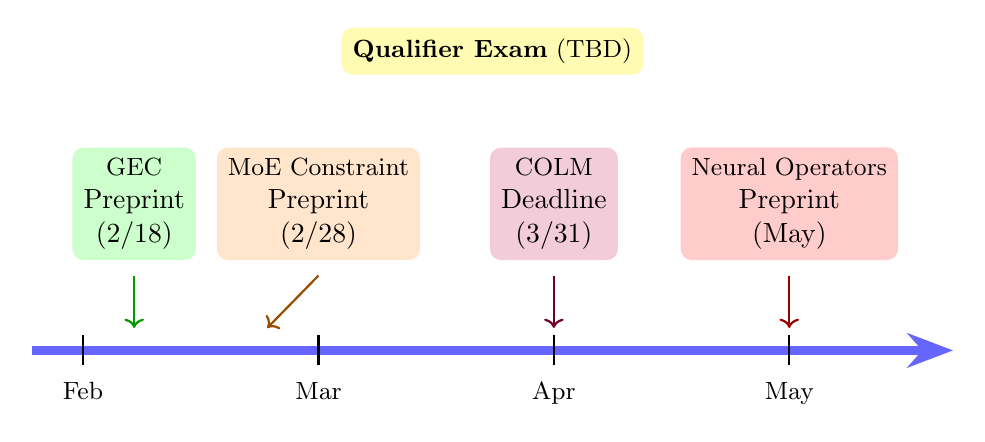
\begin{tikzpicture}[xscale=1.3, yscale=0.95]
    % Big arrow at bottom
    \draw[->, >=Stealth, line width=3pt, blue!60] (0,0) -- (9,0);
    
    % Time markers
    \foreach \x/\t in {0.5/Feb, 2.8/Mar, 5.1/Apr, 7.4/May} {
        \draw[thick] (\x, -0.2) -- (\x, 0.2);
        \node[below] at (\x, -0.3) {\small \t};
    }
    
    % Projects on top
    \node[above, align=center, fill=green!20, rounded corners, inner sep=4pt] at (1.0, 1.2) {\small GEC\\Preprint\\(2/18)};
    \node[above, align=center, fill=orange!20, rounded corners, inner sep=4pt] at (2.8, 1.2) {\small MoE Constraint\\Preprint\\(2/28)};
    \node[above, align=center, fill=purple!20, rounded corners, inner sep=4pt] at (5.1, 1.2) {\small COLM\\Deadline\\(3/31)};
    \node[above, align=center, fill=red!20, rounded corners, inner sep=4pt] at (7.4, 1.2) {\small Neural Operators\\Preprint\\(May)};
    
    % Qualifier at top (no specific time)
    \node[align=center, fill=yellow!30, rounded corners, inner sep=4pt] at (4.5, 4.0) {\small \textbf{Qualifier Exam} (TBD)};
    
    % Arrows pointing down
    \draw[->, thick, green!60!black] (1.0, 1.0) -- (1.0, 0.3);
    \draw[->, thick, orange!60!black] (2.8, 1.0) -- (2.3, 0.3);
    \draw[->, thick, purple!60!black] (5.1, 1.0) -- (5.1, 0.3);
    \draw[->, thick, red!60!black] (7.4, 1.0) -- (7.4, 0.3);
\end{tikzpicture}
\end{frame}

%% Slide 3/25: GEC Overview - What to do before preprint
\begin{frame}{GEC: Before Preprint (Feb 18)}
\begin{enumerate}
    \item \textbf{Experiments:} Warmup schedules, routing stability, visualizations
    \item \textbf{Code:} Cleanup for open source
    \item \textbf{Paper:} Redo Figure 1, write up results
\end{enumerate}
\end{frame}

%% Slide 4/25: ICLR Workshop opportunity
\begin{frame}{ICLR Workshop: Test-Time Updates}
\textbf{Deadline: Feb 6 (tomorrow!)} Non-archival, 4-page.

\vspace{0.5cm}
\textbf{Relevant track:} ``Dynamic Architectures''
\begin{itemize}
    \item Dynamically allocating compute, MoD, early-exit
\end{itemize}

\vspace{0.3cm}
\textbf{Idea:} ``Autoregressive Inference for Expert Choice''
\begin{itemize}
    \item EMA threshold $=$ test-time adaptation of routing
\end{itemize}

\vspace{0.5cm}
\textbf{Question:} Should we submit?
\end{frame}

%% Slide 5/25: GEC Experiment - Warmup Schedules
\begin{frame}{GEC Exp: Warmup Schedules}
\textbf{Experiment:} Vary warmup schedule for cutoff EMA

\vspace{0.3cm}
\centering

\includegraphics[width=0.75\textwidth]{figures/figures/ablations/warmup/warmup_a_cutoff.pdf}

\vspace{0.2cm}
\textbf{Goal:} Find optimal warmup to reduce early-stage oscillations
\end{frame}

%% Slide 6/25: GEC Experiment - Routing Stability
\begin{frame}{GEC Exp: Routing Stability}
\textbf{Hypothesis:} EC more stable than TC

\vspace{0.5cm}
\textbf{Experiment:} Correlation of routing between checkpoints
\[
\text{Stability} = \text{Corr}(A^{(t)}, A^{(t+\Delta)})
\]

\vspace{0.3cm}
Higher correlation $\Rightarrow$ more stable routing
\end{frame}

%% Slide 7/25: GEC Experiment - Visualizations
\begin{frame}{GEC Exp: Visualizations}
\begin{enumerate}
    \item \textbf{Router logit distribution} over training
    \item \textbf{Fanout vs Loss:} Do hard tokens get more experts?
    \item \textbf{Expert specialization:} Domain/topic clustering
\end{enumerate}
\end{frame}

%% Slide 8/25: GEC Code - Open Source
\begin{frame}{GEC: Open Source}
\begin{itemize}
    \item[$\square$] Code cleanup
    \item[$\square$] Documentation
    \item[$\square$] Example scripts
    \item[$\square$] Checkpoints
\end{itemize}

\vspace{0.3cm}
\textbf{Target:} Release with preprint
\end{frame}

%% Slide 9/25: GEC - Illustration Figure
\begin{frame}{GEC: Redo Figure 1}
\begin{itemize}
    \item TC vs EC vs GEC comparison
    \item Global batch routing
    \item EMA threshold mechanism
\end{itemize}
\end{frame}

%% Slide 10/25: MoE Constraint - Title
\begin{frame}{MoE as Constraint Optimization}
\centering
\vspace{1cm}
{\Large \textbf{Position Paper:}}

\vspace{0.5cm}
{\large MoE Load Balancing Should Be Treated as a Constraint Optimization Problem}

\vspace{1cm}
Target: NeurIPS 2026 Position Track
\end{frame}

%% Slide 11/25: MoE Constraint - Problem Setup
\begin{frame}{MoE Constraint: Problem Formulation}
\begin{align*}
\max_{z \in \{0,1\}^{N \times GE}} \quad & \sum_{t=1}^N \sum_{i=1}^{GE} z_{t,i}\, r_{t,i} \\
\text{s.t.} \quad
& \sum_{i=1}^{GE} z_{t,i} = G, \quad \forall t \qquad (\text{Sparsity}) \\
& \sum_{t=1}^{N} z_{t,i} = k, \quad \forall i \qquad (\text{Load balance})
\end{align*}
\[
k = \frac{N}{E},
\qquad
\frac{G}{GE} = \frac{1}{E},
\qquad
f_i \triangleq \frac{E}{N}\sum_{t=1}^N z_{t,i},\ \ f^*=1
\]
\end{frame}

%% Slide 12/25: MoE Constraint - Lagrangian
\begin{frame}{MoE Constraint: Lagrangian Duality}
\[
\mathcal{L}(z,\lambda)
= \sum_{t,i} z_{t,i}\, r_{t,i} - \sum_{i=1}^{GE} \lambda_i (f_i - 1)
= \sum_{t,i} z_{t,i}\, (r_{t,i} + b_i) + \sum_{i=1}^{GE}\lambda_i
\]
\[
b_i \triangleq -\frac{\lambda_i}{k},
\qquad
z_{t,i} = \mathbb{1}\!\left\{i \in \mathrm{Top}_G(r_{t,\cdot} + b)\right\}
\]
\[
\lambda_i^{(t+1)} = \lambda_i^{(t)} + \mu (f_i^{(t)} - 1)
\]
\end{frame}

%% Slide 13/25: MoE Constraint - Controller View
\begin{frame}{MoE Constraint: PID Control View}
\[
e_i^{(t)} \triangleq f_i^{(t)} - 1
\]
\[
\text{LongCat:}\quad b_i^{(t+1)} = b_i^{(t)} - \mu\, e_i^{(t)}
\]
\[
\text{DeepSeek:}\quad b_i^{(t+1)} = b_i^{(t)} - u\,\mathrm{sgn}(e_i^{(t)})
\]
\[
b_i^{(t)} = b_i^{(0)} - \mu \sum_{\tau=0}^{t-1} e_i^{(\tau)}
\ \approx\ -\mu \int_0^t e_i(\tau)\, d\tau
\]
\end{frame}

%% Slide 14/25: MoE Constraint - Methods Comparison
\begin{frame}{MoE Constraint: Methods Taxonomy}
\begin{table}
\centering
\small
\begin{tabular}{@{}lll@{}}
\toprule
\textbf{Method} & \textbf{Update Rule} & \textbf{Type} \\
\midrule
Aux Loss & $\mathcal{L}_{\text{aux}} = \alpha \sum_i e_i P_i$ & Penalty / Coupled I \\
DeepSeek & $b_i \leftarrow b_i - u\,\mathrm{sgn}(e_i)$ & Dual / I (Sign) \\
LongCat & $b_i \leftarrow b_i - \mu\, e_i$ & Dual / I (Prop.) \\
Expert Choice & $z_{t,i}=\mathbb{1}\{t\in \mathrm{Top}_k(r_{\cdot,i})\}$ & Projection \\
Sinkhorn & $z^\star = \mathrm{Sinkhorn}(r;\varepsilon)$ & Entropic OT \\
\bottomrule
\end{tabular}
\end{table}
\end{frame}

%% Slide 15/25: MoE Constraint - Expert Choice
\begin{frame}{MoE Constraint: Expert Choice}
\begin{align*}
\max_{z} \quad & \sum_{i=1}^{GE}\left(\sum_{t=1}^N z_{t,i}\, r_{t,i}\right) \\
\text{s.t.}\quad & \sum_{t=1}^N z_{t,i} = k,\quad \forall i
\end{align*}
\[
z_{t,i} = \mathbb{1}\!\left\{t \in \mathrm{Top}_k(r_{\cdot,i})\right\}
\qquad (\text{perfect load balance})
\]
\end{frame}

%% Slide 16/25: MoE Constraint - GEC Stochastic Relaxation
\begin{frame}{MoE Constraint: GEC as Stochastic Relaxation}
\[
\text{Batch EC:}\quad z_{t,i} = \mathbb{1}\!\left\{t \in \mathrm{Top}_k(r_{\cdot,i})\right\}
\]
\[
(\text{non-causal})
\]
\[
\text{GEC:}\quad \mathbb{E}_{\text{data}}\!\left[\sum_{t=1}^N z_{t,i}\right] = k,
\qquad
z_{t,i} = \mathbb{1}\!\left\{r_{t,i} > c_i\right\}
\]
\[
\Pr_{t\sim \text{data}}\!\left[r_{t,i} > c_i\right] = \frac{1}{E},
\qquad
\sum_{t=1}^N \mathbb{1}\!\left\{r_{t,i} > \hat c_i^{(t)}\right\} = k,
\qquad
c_i^{(t+1)} = \beta c_i^{(t)} + (1-\beta)\,\hat c_i^{(t)}
\]
\end{frame}

%% Slide 17/25: MoE Constraint - Sinkhorn
\begin{frame}{MoE Constraint: Sinkhorn OT}
\begin{align*}
\max_{z \ge 0}\quad
& \sum_{t,i} z_{t,i}\, r_{t,i}
+ \varepsilon \sum_{t,i} z_{t,i}\,(1-\log z_{t,i}) \\
\text{s.t.}\quad
& \sum_{i=1}^{GE} z_{t,i} = G,\ \forall t,
\qquad
\sum_{t=1}^{N} z_{t,i} = k,\ \forall i
\end{align*}
\[
z^{(0)}_{t,i} = \exp(r_{t,i}/\varepsilon)
\]
\[
z^{(m+\frac{1}{2})}_{t,i}
= z^{(m)}_{t,i}\cdot \frac{G}{\sum_{i'} z^{(m)}_{t,i'}}
\qquad
z^{(m+1)}_{t,i}
= z^{(m+\frac{1}{2})}_{t,i}\cdot \frac{k}{\sum_{t'} z^{(m+\frac{1}{2})}_{t',i}}
\]
\end{frame}

%% Slide 18/25: MoE Constraint - Conclusion
\begin{frame}{MoE Constraint: Key Takeaways}
\[
\max_{z\in\{0,1\}^{N\times GE}} \ \sum_{t,i} z_{t,i}\, r_{t,i}
\quad \text{s.t.}\quad
\sum_i z_{t,i}=G,\ \sum_t z_{t,i}=k
\]
\[
\text{Dual:}\quad \Delta b_i = -\mu(f_i-1)
\qquad
\text{EC:}\quad z_{t,i}=\mathbb{1}\{t\in \mathrm{Top}_k(r_{\cdot,i})\}
\]
\[
\text{GEC:}\quad z_{t,i}=\mathbb{1}\{r_{t,i}>c_i\}
\qquad
\text{Sinkhorn:}\quad z^\star = \arg\max_{z\ge 0}\ \langle z,r\rangle + \varepsilon \sum_{t,i} z_{t,i}(1-\log z_{t,i})
\]
\end{frame}

%% Slide 19/25: Neural Operators
\begin{frame}{Neural Operators}
\centering
\vspace{1cm}
{\Large \textit{(Separate slide deck)}}

\vspace{1cm}
\textbf{Topic:} All Sequential Models are Neural Operators

\vspace{0.5cm}
Target: May preprint, NeurIPS Position Track
\end{frame}

%% Slide 20/25: Paper Ideas
\begin{frame}{Paper Ideas}
\textbf{Bandwidth for one more paper this semester}

\vspace{0.5cm}
\textbf{Target:} COLM 2026 (deadline: Mar 31)

\vspace{0.5cm}
\textbf{Potential topics:}
\begin{itemize}
    \item TBD -- discuss next meeting
\end{itemize}
\end{frame}

%% Slide 21/25: Qualifier Exam Overview
\begin{frame}{Qualifier Exam: Overview}
\textbf{From CSE PhD Handbook:}

\vspace{0.3cm}
\begin{itemize}
    \item \textbf{Timeline:} Recommended by end of Year 2
    \begin{itemize}
        \item Must complete by end of Year 3
    \end{itemize}
    
    \vspace{0.2cm}
    \item \textbf{Components:}
    \begin{enumerate}
        \item Qualifier Project (research activity + written document)
        \item Qualifier Exam (oral presentation)
    \end{enumerate}
    
    \vspace{0.2cm}
    \item \textbf{Committee:} 3 faculty members with CSE appointment
    
    \vspace{0.2cm}
    \item \textbf{Two attempts allowed}
\end{itemize}
\end{frame}

%% Slide 22/25: Qualifier Project
\begin{frame}{Qualifier Exam: Project}
\textbf{Qualifier Project Requirements:}

\vspace{0.3cm}
\begin{itemize}
    \item Substantial research activity
    \item Flexible format:
    \begin{itemize}
        \item Original research project
        \item Survey paper
        \item Replication study
        \item Substantial software
    \end{itemize}
    \item Written document summarizing results
\end{itemize}

\vspace{0.5cm}
\textbf{Skills assessed:}
\begin{itemize}
    \item Independent research (Goal 1.b)
    \item Written communication (Goal 3)
\end{itemize}
\end{frame}

%% Slide 23/25: Qualifier Exam Details
\begin{frame}{Qualifier Exam: Oral Presentation}
\textbf{Format:}
\begin{itemize}
    \item Public oral presentation ($\sim$30 min)
    \item Q\&A from committee and audience ($\sim$30 min)
    \item Optional closed-door questions
    \item Committee deliberation
\end{itemize}

\vspace{0.5cm}
\textbf{Skills assessed:}
\begin{itemize}
    \item Oral communication (Goal 3)
    \item Technical proficiency (Goal 1.b, 2.a, 2.b)
\end{itemize}
\end{frame}

%% Slide 24/25: Qualifier Topic Discussion
\begin{frame}{Qualifier: Topic Discussion}
\textbf{Question:} Which topic for qualifier?

\vspace{0.5cm}
\begin{columns}
\begin{column}{0.48\textwidth}
\textbf{Option A: GEC}
\begin{itemize}
    \item More mature codebase
    \item Experiments underway
    \item Clear contribution
\end{itemize}
\end{column}
\begin{column}{0.48\textwidth}
\textbf{Option B: MoE Constraint}
\begin{itemize}
    \item Broader scope
    \item Position paper angle
    \item Unifying framework
\end{itemize}
\end{column}
\end{columns}

\vspace{0.5cm}
\textbf{Discussion:} What would professor recommend?
\end{frame}

%% Slide 25/25: PhD Timeline
\begin{frame}{PhD Program Timeline}
\begin{table}
\centering
\small
\begin{tabular}{@{}lll@{}}
\toprule
\textbf{Year} & \textbf{Milestone} & \textbf{Status} \\
\midrule
1 & Core courses (CSE 406, 411, 440) & \checkmark \\
1--3 & Breadth courses (3 areas) & \checkmark \\
2--3 & \textbf{Qualifier} & \textcolor{orange}{In progress} \\
3 & Admission to candidacy & -- \\
3 & General exam & -- \\
3--5 & Dissertation + Defense & -- \\
\bottomrule
\end{tabular}
\end{table}

\vspace{0.3cm}
\textbf{Note:} Must complete qualifier by end of Year 3
\end{frame}

%%%%%%%%%%% Jan 08 progress update %%%%%%%%%%%
%% Slide 1: January 08 Overview
\begin{frame}{January 08 Progress Overview}
\begin{enumerate}
    \item \textbf{Token Choice MoE (TC-MoE)}
    \item \textbf{Training data migration: 10B $\rightarrow$ 37B tokens}
    \item \textbf{Core-Eval setup (nanochat, DCLM)}
    \item \textbf{Infra: UFIT cluster access}
    \item \textbf{Reading: Qwen global-batch load-balancing loss (LBL)}
    \item \textbf{Paper plan + position-paper angle}
\end{enumerate}
\end{frame}

%% Slide 2: Token Choice MoE
\begin{frame}{Token Choice MoE (TC-MoE)}
\begin{itemize}
    \item Standard MoE routing: each \textbf{token} selects top-$k$ experts (with capacity constraints)
    \item Baselines to include: \textbf{aux loss} vs \textbf{aux-loss-free} (DeepSeek-style)
    \item Goal: compare against \textbf{Expert Choice} / \textbf{Global Expert Choice} routing
\end{itemize}
\end{frame}

%% Slide 3: Data Migration
\begin{frame}{Migration: Karpathy Dataset (37B vs 10B)}
\begin{itemize}
    \item Switch training data from \textbf{10B} tokens to \textbf{37B} tokens
    \item Motivation: stronger scaling signal + reduce overfitting to small data
    \item Checklist: preprocessing/sharding, packing, and sanity-check token counts
\end{itemize}
\end{frame}

%% Slide 4: Core Eval + Cluster
\begin{frame}{Core-Eval Setup + UFIT Cluster}
\textbf{Core-Eval}
\begin{itemize}
    \item Align evaluation pipeline with \textbf{nanochat} and \textbf{DCLM} references
    \item Standardize reporting: training loss + core-eval suite
\end{itemize}

\vspace{0.4cm}
\textbf{Infra}
\begin{itemize}
    \item Logged onto \textbf{UFIT cluster}; environment ready for runs
\end{itemize}
\end{frame}

%% Slide 5-6: Qwen Global LBL (import figures)
\begin{frame}[plain]
\centering
\includegraphics[height=0.95\textheight]{figures/figures/_archive_slides/papers/global_lbl/fig1b_expert_frequency_heatmaps.png}
\end{frame}

\begin{frame}[plain]
\centering
\includegraphics[height=0.95\textheight]{figures/figures/_archive_slides/papers/global_lbl/table2_lbl_token_ablation.png}
\end{frame}

%% Slide 7-12: Plan for paper
\begin{frame}{Plan: Status + Motivation}
\begin{enumerate}
    \item \textbf{Methods:} done
    \item \textbf{Gap:} many MoE papers report fewer experiments than other arch papers
    \item \textbf{Example:} DeepSeek aux-loss-free mainly reports perplexity
\end{enumerate}
\end{frame}

\begin{frame}{Plan: Experiments (Small Scale)}
\textbf{Model:} GPT-2 Small
\vspace{0.3cm}
\begin{itemize}
    \item TC-MoE (aux loss)
    \item TC-MoE (DeepSeek loss-free)
    \item Expert Choice (vary batch size)
    \item GEC top-$k$
    \item GEC threshold (vary capacity)
\end{itemize}
\end{frame}

\begin{frame}{Plan: Experiments (Medium Scale)}
\textbf{Model:} nanochat-d20 (3.4B total / 0.5B active)
\vspace{0.3cm}
\begin{itemize}
    \item TC-MoE (aux loss)
    \item TC-MoE (DeepSeek loss-free)
    \item Expert Choice (vary batch size)
    \item GEC top-$k$
    \item GEC threshold (vary capacity)
\end{itemize}
\end{frame}

\begin{frame}{Compute Cost Estimate}
\begin{itemize}
    \item Budget target: \textbf{8$\times$ B200} for a \textbf{few days} is sufficient for the main study
    \item Example: nanochat-d20 (3.4B total / 0.5B active) run takes \textbf{$\sim$4 hours} on \textbf{8$\times$ B200}
\end{itemize}
\end{frame}

\begin{frame}{Plan: What to Report}
\begin{itemize}
    \item \textbf{Loss:} training + validation curves
    \item \textbf{Core-Eval:} standardized benchmark suite results
\end{itemize}
\end{frame}

\begin{frame}{Plan: Explanation / Ablations}
\begin{itemize}
    \item Plot expert activation patterns by \textbf{category / benchmark}
    \item Test whether global routing gains come from \textbf{specialization} vs \textbf{variance reduction} (Qwen-style)
\end{itemize}
\end{frame}

\begin{frame}{Plan: Paper Structure (Draft)}
\begin{itemize}
    \item Methods (done)
    \item Experimental matrix (small + medium scale)
    \item Core-eval + loss reporting
    \item Mechanistic analysis / ablations
\end{itemize}
\end{frame}

%% Slide 13: Position paper
\begin{frame}{Position Paper: Constraint Optimization View}
\begin{itemize}
    \item View routing/load-balancing as \textbf{constrained optimization}
    \item Objective: minimize loss; constraints: expert capacity, balance, compute budget
\end{itemize}
\end{frame}

%%%%%%%%%%% Dec 17 progress update %%%%%%%%%%%

%% Slide: December 17 Overview
\begin{frame}{December 17 Progress Overview}
\begin{enumerate}
    \item \textbf{Zero Initialization}
    \begin{itemize}
        \item Improves loss significantly
        \item Stabilizes capacity overflow/underflow
    \end{itemize}

    \item \textbf{Expert Parallelism (EP) Implementation}
    \begin{itemize}
        \item Memory: 23 GB $\to$ 18 GB per GPU
        \item 8$\times$ batch size (128k tokens)
    \end{itemize}

    \item \textbf{Finding: First Layer Dense}
    \begin{itemize}
        \item L0 routing unstable $\to$ use dense MLP
        \item Prior art: DeepSeek-MoE, Kimi
    \end{itemize}

    \item \textbf{Finding: EMA Stability Trade-off}
    \begin{itemize}
        \item 0.999 EMA more stable but causes delay
        \item Future: Holt's linear, Double EMA, Adaptive EMA
    \end{itemize}

    \item \textbf{Experiment Results (5.0--5.2)}
    \begin{itemize}
        \item Best: Capacity + FLD + 0.999 EMA (loss: 3.405)
    \end{itemize}
\end{enumerate}
\end{frame}

%% -------- Zero Init & Capacity --------

\begin{frame}{Zero Initialization: Loss Improvement}
\textbf{Zero init improves loss significantly}

\vspace{0.3cm}
\centering

\includegraphics[width=0.85\textwidth]{figures/figures/_archive_slides/figs/eval_loss_zero_init.png}
\end{frame}

\begin{frame}{Capacity Constraints: Overflow}
\textbf{Overflow rate with zero init}

\vspace{0.3cm}
\centering

\includegraphics[width=0.85\textwidth]{figures/figures/_archive_slides/figs/capacity_overflow_zeroinit_comparison.png}
\end{frame}

\begin{frame}{Capacity Constraints: Underflow}
\textbf{Underflow rate with zero init}

\vspace{0.3cm}
\centering

\includegraphics[width=0.85\textwidth]{figures/figures/_archive_slides/figs/capacity_underflow_zeroinit_comparison.png}
\end{frame}

\begin{frame}{LR Schedule and Capacity}
\textbf{Overflow/underflow drop when LR decay begins (step 15k)}

\vspace{0.3cm}
\centering

\includegraphics[width=0.85\textwidth]{figures/figures/_archive_slides/figs/train_lr_schedule.png}
\end{frame}

%% -------- Training Diagnostics --------

\begin{frame}{Training: Gradient Norm}
\textbf{Gradient norm during training}

\vspace{0.3cm}
\centering

\includegraphics[width=0.85\textwidth]{figures/figures/_archive_slides/figs/train_grad_norm.png}
\end{frame}

%% -------- Expert Parallelism --------

\begin{frame}{Expert Parallelism (EP) Implementation}
\textbf{Goal:} Scale batch size via distributed expert computation

\vspace{0.5cm}
\textbf{Memory savings:}
\begin{itemize}
    \item Before EP: \textbf{23 GB} per GPU
    \item After EP: \textbf{18 GB} per GPU
    \item Savings: 5 GB (\textbf{22\% reduction})
\end{itemize}

\vspace{0.5cm}
\textbf{This enables:}
\begin{itemize}
    \item Larger model capacity
    \item More experts per layer
    \item Bigger batch sizes
\end{itemize}
\end{frame}

\begin{frame}{EP Benefits}
\textbf{Scaling advantages:}
\begin{itemize}
    \item 8$\times$ effective batch size (128k tokens)
    \item Better gradient estimates from global routing
    \item Each expert sees tokens from all GPUs
\end{itemize}

\vspace{0.5cm}
\textbf{Implementation:}
\begin{itemize}
    \item All-to-all communication for token dispatch
    \item All-to-all communication for output combine
    \item Overlaps with computation where possible
\end{itemize}
\end{frame}

%% -------- First Layer Dense: Problem --------

\begin{frame}{L0 Problem: Wild Oscillations}
\textbf{Problem:} L0 routing exhibits unstable behavior

\vspace{0.3cm}
Cutoff values oscillate wildly: 0 $\to$ 18 $\to$ 10 $\to$ 18...

\vspace{0.3cm}
\centering

\includegraphics[width=0.85\textwidth]{figures/figures/_archive_slides/figs/routing_layers_L0_E0_cutoff.png}
\end{frame}

\begin{frame}{L0 Problem: Cutoff EMA}
\textbf{Cutoff EMA also shows instability}

\vspace{0.3cm}
\centering

\includegraphics[width=0.85\textwidth]{figures/figures/_archive_slides/figs/routing_layers_L0_E0_cutoff_ema.png}
\end{frame}

\begin{frame}{L0 Problem: Raw Expert Usage}
\textbf{Raw usage spikes when cutoff drops}

\vspace{0.3cm}
\centering

\includegraphics[width=0.85\textwidth]{figures/figures/_archive_slides/figs/routing_layers_L0_E0_raw_usage.png}
\end{frame}

%% -------- First Layer Dense: Solution --------

\begin{frame}{Solution: First Layer Dense}
\textbf{Solution:} Use dense MLP for first layer (no routing)

\vspace{0.5cm}
\textbf{Prior art:}
\begin{itemize}
    \item \textbf{DeepSeek-MoE}: Dense layers before MoE transition
    \item \textbf{Kimi}: First-layer-dense as standard practice
\end{itemize}

\vspace{0.5cm}
\textbf{Why it works:}
\begin{enumerate}
    \item Early layers learn general representations
    \item No specialization needed at L0
    \item Routing decisions harder with unstable inputs
\end{enumerate}
\end{frame}

\begin{frame}{First Layer Dense: Cutoff Stabilized}
\textbf{With first-layer-dense, L0 issues eliminated}

\vspace{0.3cm}
\centering

\includegraphics[width=0.85\textwidth]{figures/figures/_archive_slides/figs/routing_L0_E0_cutoff_zeroinit.png}
\end{frame}

\begin{frame}{First Layer Dense: Loss Comparison}
\textbf{FLD achieves comparable loss to baseline}

\vspace{0.3cm}
\centering

\includegraphics[width=0.85\textwidth]{figures/figures/_archive_slides/figs/eval_loss_topk_fld_vs_zeroinit.png}
\end{frame}

%% -------- Later Layers: Stable --------

\begin{frame}{Later Layers: L4 Cutoff EMA}
\textbf{L4 shows stable behavior (small oscillations)}

\vspace{0.3cm}
\centering

\includegraphics[width=0.85\textwidth]{figures/figures/_archive_slides/figs/routing_layers_L4_E0_cutoff_ema.png}
\end{frame}

\begin{frame}{Later Layers: L6 Cutoff EMA}
\textbf{L6 also stable}

\vspace{0.3cm}
\centering

\includegraphics[width=0.85\textwidth]{figures/figures/_archive_slides/figs/routing_layers_L6_E0_cutoff_ema.png}
\end{frame}

%% -------- Experiment Results --------

\begin{frame}{Experiment Results: Summary}
\textbf{Three experiments with first-layer-dense (FLD):}

\vspace{0.3cm}
\begin{table}
\centering
\begin{tabular}{@{}llc@{}}
\toprule
\textbf{Exp} & \textbf{Config} & \textbf{Eval Loss @ 19k} \\
\midrule
5.0 & Topk + FLD + 0.99 EMA & 3.40737 \\
5.1 & Capacity + FLD + 0.993 EMA & 3.40714 \\
5.2 & Capacity + FLD + 0.999 EMA & \textbf{3.40456} \\
\bottomrule
\end{tabular}
\end{table}

\vspace{0.5cm}
\textbf{Key finding:} Capacity constraints + slower EMA achieves best loss
\end{frame}

\begin{frame}{Experiment Results: Loss Curves}
\textbf{Comparing 5.0, 5.1, 5.2}

\vspace{0.3cm}
\centering

\includegraphics[width=0.85\textwidth]{figures/figures/_archive_slides/figs/eval_loss_fld_comparison.png}
\end{frame}

%% -------- EMA Trade-off --------

\begin{frame}{EMA Stability vs Responsiveness}
\textbf{Problem:} Cutoff EMA oscillates with 0.99 decay

\vspace{0.5cm}
\textbf{Current solution:} Longer EMA (0.999)
\begin{itemize}
    \item[\textcolor{green}{$\checkmark$}] More stable cutoffs
    \item[\textcolor{green}{$\checkmark$}] Eliminates periodic oscillations
    \item[\textcolor{red}{$\times$}] Causes delay in tracking distribution shifts
\end{itemize}
\end{frame}

\begin{frame}{EMA Comparison: Overflow Rate}
\textbf{0.993 vs 0.999 EMA decay}

\vspace{0.3cm}
\centering

\includegraphics[width=0.85\textwidth]{figures/figures/_archive_slides/figs/capacity_overflow_ema_comparison.png}
\end{frame}

\begin{frame}{EMA Comparison: Underflow Rate}
\textbf{0.993 vs 0.999 EMA decay}

\vspace{0.3cm}
\centering

\includegraphics[width=0.85\textwidth]{figures/figures/_archive_slides/figs/capacity_underflow_ema_comparison.png}
\end{frame}

\begin{frame}{EMA Alternatives}
\textbf{Potential alternatives to simple EMA:}

\vspace{0.5cm}
\begin{enumerate}
    \item \textbf{Holt's Linear Trend}
    \begin{itemize}
        \item Tracks both level and trend
        \item Better at following systematic changes
    \end{itemize}

    \item \textbf{Double EMA}
    \begin{itemize}
        \item Apply EMA twice to reduce lag
        \item Maintains smoothness
    \end{itemize}

    \item \textbf{Adaptive EMA}
    \begin{itemize}
        \item Adjust decay based on recent variance
        \item High variance $\to$ faster response
    \end{itemize}
\end{enumerate}
\end{frame}

%%%%%%%%%%% Nov 19 progress update %%%%%%%%%%%

\begin{frame}{Progress Report}

\textbf{Two major accomplishments this week:}

\vspace{0.5cm}

\begin{itemize}
    \item \textbf{Papersearch MCP}
    \item \textbf{Scatter Kernel}
\end{itemize}

\end{frame}

\begin{frame}{Papersearch MCP}

\textbf{Overview:}
\begin{itemize}
    \item MCP server for searching and downloading academic papers
    \item Seamless integration with Claude for literature review workflows
\end{itemize}

\vspace{0.5cm}

\textbf{Configuration:}
\begin{itemize}
    \item \textbf{Restricted Sources:}
    \begin{itemize}
        \item \textbf{arXiv}
        \item \textbf{Semantic Scholar}
    \end{itemize}
    \item Focused on ML/AI research papers
\end{itemize}

\vspace{0.5cm}

\textbf{Repository:} \url{https://github.com/openags/paper-search-mcp}

\end{frame}

\begin{frame}{Claude SubAgents}
\begin{center}
    \includegraphics[width=0.9\textwidth]{figures/figures/_archive_slides/claude_subagents.png}
\end{center}

\end{frame}

\begin{frame}{Architecture Comparison}
    \begin{columns}
        \begin{column}{0.48\textwidth}
            \centering
            \textbf{Claude SubAgents (Current)}\\
            \vspace{0.3cm}
            \scalebox{0.65}{
            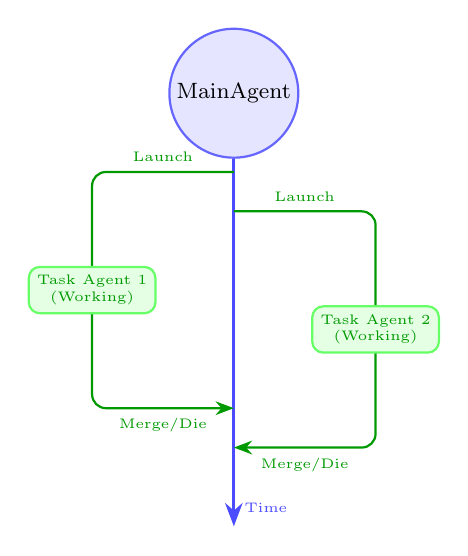
\begin{tikzpicture}[
                node distance=1.5cm,
                font=\footnotesize,
                main_flow/.style={->, >=Stealth, very thick, blue!70},
                sub_flow/.style={->, >=Stealth, thick, green!60!black, rounded corners=5pt},
                task_node/.style={rectangle, fill=green!10, draw=green!60, rounded corners, align=center, font=\tiny, inner sep=3pt},
                label_text/.style={font=\tiny, color=black!70, align=center}
            ]
                % Main Agent Timeline
                \node[circle, fill=blue!10, draw=blue!60, thick, inner sep=2pt] (start) at (0,0) {Main\\Agent};
                \coordinate (end) at (0,-5.5);
                \draw[main_flow] (start) -- node[pos=0.95, right, font=\tiny] {Time} (end);

                % Subagent 1 (Left)
                \coordinate (launch1) at (0,-1.0);
                \coordinate (return1) at (0,-4.0);
                \draw[sub_flow] (launch1) -- ++(-1.8, 0) node[midway, above, font=\tiny] {Launch}
                    -- node[midway, task_node] {Task Agent 1\\(Working)} ++(0, -3.0) 
                    -- (return1) node[midway, below, font=\tiny] {Merge/Die};

                % Subagent 2 (Right)
                \coordinate (launch2) at (0,-1.5);
                \coordinate (return2) at (0,-4.5);
                \draw[sub_flow] (launch2) -- ++(1.8, 0) node[midway, above, font=\tiny] {Launch}
                    -- node[midway, task_node] {Task Agent 2\\(Working)} ++(0, -3.0) 
                    -- (return2) node[midway, below, font=\tiny] {Merge/Die};

            \end{tikzpicture}
            }
            \vspace{0.2cm}
            \footnotesize
            \begin{itemize}
                \item Hierarchical (Fork-Join)
                \item Ephemeral Workers
                \item Main agent aggregates results
            \end{itemize}
        \end{column}

        \begin{column}{0.48\textwidth}
            \centering
            \textbf{Herd of Agents (Previous)}\\
            \vspace{0.3cm}
            \scalebox{0.65}{
            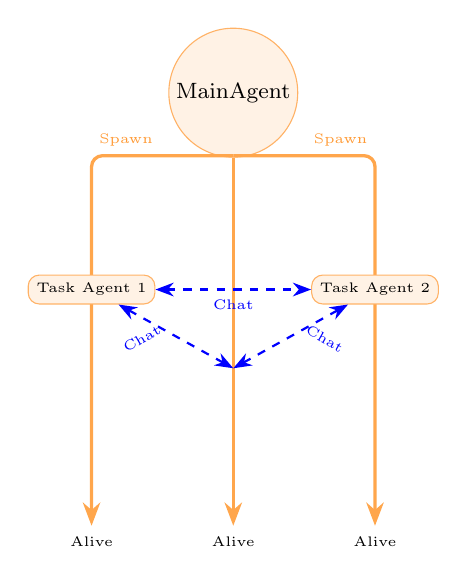
\begin{tikzpicture}[
                node distance=1.0cm,
                font=\footnotesize,
                flow/.style={->, >=Stealth, very thick, orange!70},
                chat/.style={<->, >=Stealth, dashed, blue, thick},
                task_node/.style={rectangle, fill=orange!10, draw=orange!60, rounded corners, align=center, font=\tiny, inner sep=3pt},
                label_text/.style={font=\tiny, color=black!70}
            ]
                % Main Agent
                \node[circle, fill=orange!10, draw=orange!60, inner sep=2pt] (startA) at (0,0) {Main\\Agent};
                \draw[flow] (startA) -- (0,-5.5) node[below, black, font=\tiny] {Alive};

                % Task Agent 1 (Left)
                \coordinate (spawn1) at (0,-0.8);
                \draw[flow, rounded corners] (spawn1) -- (-1.8,-0.8) -- (-1.8,-5.5) node[below, black, font=\tiny] {Alive};
                \node[task_node] (t1) at (-1.8,-2.5) {Task Agent 1};
                \node[above left, font=\tiny, orange!80] at (-0.9,-0.8) {Spawn};

                % Task Agent 2 (Right)
                \coordinate (spawn2) at (0,-0.8);
                \draw[flow, rounded corners] (spawn2) -- (1.8,-0.8) -- (1.8,-5.5) node[below, black, font=\tiny] {Alive};
                \node[task_node] (t2) at (1.8,-2.5) {Task Agent 2};
                \node[above right, font=\tiny, orange!80] at (0.9,-0.8) {Spawn};

                % Chat Interaction - Triangle
                \draw[chat] (0,-3.5) -- node[midway, above left, font=\tiny, rotate=30] {Chat} (t1);
                \draw[chat] (0,-3.5) -- node[midway, above right, font=\tiny, rotate=-30] {Chat} (t2);
                \draw[chat] (t1) -- node[midway, below, font=\tiny] {Chat} (t2);

            \end{tikzpicture}
            }
            \vspace{0.2cm}
            \footnotesize
            \begin{itemize}
                \item Decentralized (Network)
                \item Persistent Agents
                \item Peer-to-Peer Chat
            \end{itemize}
        \end{column}
    \end{columns}
    
    \vspace{0.5cm}
    \hrule
    \vspace{0.1cm}
    \tiny \url{https://github.com/MasterGodzilla/Herd_of_Agents}
\end{frame}

\begin{frame}{Example 1: Parallel Agents Research}

\begin{itemize}
    \item Launch subagents for search paper, read, and summarize
    \item Launch codex mcp for thinking hard problems (\textcolor{red}{TODO})
    \item Summarization
\end{itemize}

\end{frame}

\begin{frame}{Example 2: Data Labeling for Idea Flow}
\begin{itemize}
    \item \textbf{Goal:} Automate extraction of Idea Flow (inheritance of ideas) from papers
    \item \textbf{Method:} Multi-agent System (Claude Agents)
    \item \textbf{Workflow:}
    \begin{itemize}
        \item \textbf{Input:} Graph image or topic
        \item \textbf{Subagents:} Research papers, download PDFs, generate markdown reviews
        \item \textbf{Relationship Extraction:} Identify Extension vs. Motivation edges
        \item \textbf{Output:} Structured JSON (nodes, edges), BibTeX, and interactive visualization
    \end{itemize}
    \item \textbf{Innovation:} Automated subagents handle specific tasks to build citation graph
\end{itemize}
\end{frame}

\begin{frame}{Labeling Frontend}
\centering
\textit{(Screenshot placeholder)}
\end{frame}

\begin{frame}{Scatter Backward Kernel: Math \& Memory}

\textbf{Mathematical Formulation:}
\begin{itemize}
    \item \textbf{Forward:} $y_t = \sum_{i \in \mathcal{E}_t} w_i \cdot x_i$
    \item \textbf{Backward (Expert Gradients):} $\frac{\partial L}{\partial x_i} = \frac{\partial L}{\partial y_t} \cdot w_i$
    \item \textbf{Backward (Weight Gradients):} $\frac{\partial L}{\partial w_i} = \langle \frac{\partial L}{\partial y_t}, x_i \rangle$
\end{itemize}

\vspace{0.3cm}

\textbf{Key Optimizations:}
\begin{itemize}
    \item \textbf{Token-Parallelism:} One thread block per token $t$, iterating over contributing experts. Avoids atomic adds (unlike expert-parallel approaches).
    \item \textbf{L1 Reuse:} $\text{grad\_out}[t]$ is loaded once into L1 cache/registers and reused for all contributing experts.
    \item \textbf{Fused Kernel:} Computes both $\nabla x$ and $\nabla w$ in a single pass, minimizing memory bandwidth.
    \item \textbf{Deterministic:} Output is deterministic (no race conditions).
\end{itemize}

\end{frame}

\begin{frame}{Scatter Backward: Memory Flow}
\begin{center}
\scalebox{0.75}{
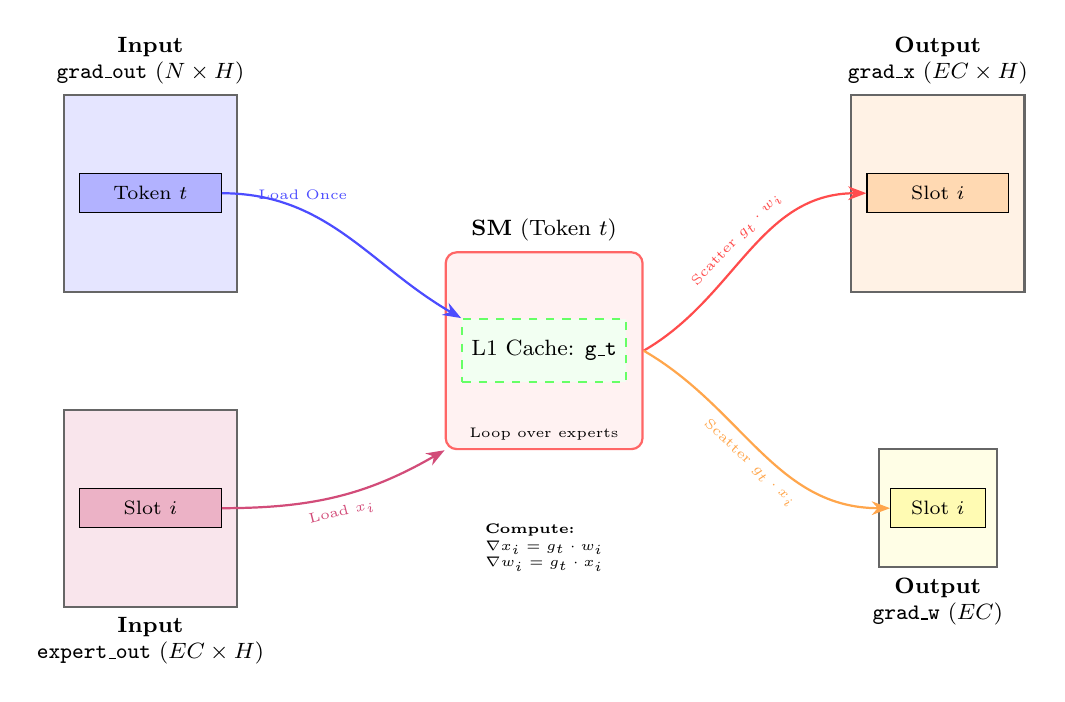
\begin{tikzpicture}[
    node distance=1.0cm,
    font=\footnotesize,
    memory_block/.style={rectangle, draw=black!60, fill=blue!5, thick, minimum width=2.2cm, minimum height=3.0cm, align=center},
    compute_block/.style={rectangle, draw=red!60, fill=red!5, thick, rounded corners, minimum width=2.5cm, minimum height=2.5cm, align=center},
    cache_block/.style={rectangle, draw=green!60, fill=green!5, thick, dashed, minimum width=2.0cm, minimum height=0.8cm, align=center},
    inner_node/.style={rectangle, draw=black, minimum width=1.8cm, minimum height=0.5cm, font=\scriptsize, fill=white},
    flow_arrow/.style={->, >=Stealth, thick, blue!70},
    label_text/.style={font=\scriptsize, color=black!70}
]

% Left Top: grad_out (Input)
\node[memory_block, fill=blue!10, minimum height=2.5cm, label={[align=center]above:\textbf{Input}\\ \texttt{grad\_out} $(N \times H)$}] (grad_out) at (0, 2.0) {};
\node[inner_node, fill=blue!30] (grad_out_t) at (grad_out.center) {Token $t$};

% Left Bottom: expert_out (Input)
\node[memory_block, fill=purple!10, minimum height=2.5cm, label={[align=center]below:\textbf{Input}\\ \texttt{expert\_out} $(EC \times H)$}] (expert_out) at (0, -2.0) {};
\node[inner_node, fill=purple!30] (expert_slot) at (expert_out.center) {Slot $i$};

% Middle: SM
\node[compute_block, label={[align=center]above:\textbf{SM} (Token $t$)}] (sm) at (5.0, 0) {};
\node[cache_block] (l1) at (sm.center) {L1 Cache: \texttt{g\_t}};
\node[font=\tiny, anchor=south] at (sm.south) {Loop over experts};

% Right Top: grad_x (Output)
\node[memory_block, fill=orange!10, minimum height=2.5cm, label={[align=center]above:\textbf{Output}\\ \texttt{grad\_x} $(EC \times H)$}] (grad_x) at (10, 2.0) {};
\node[inner_node, fill=orange!30] (grad_x_slot) at (grad_x.center) {Slot $i$};

% Right Bottom: grad_w (Output - Small)
\node[memory_block, fill=yellow!10, minimum height=1.5cm, minimum width=1.5cm, label={[align=center]below:\textbf{Output}\\ \texttt{grad\_w} $(EC)$}] (grad_w) at (10, -2.0) {};
\node[inner_node, fill=yellow!30, minimum width=1.2cm] (grad_w_slot) at (grad_w.center) {Slot $i$};

% Arrows
% Load grad_out
\draw[flow_arrow] (grad_out_t.east) to[out=0,in=150] node[above, font=\tiny, pos=0.3] {Load Once} (l1.north west);

% Load expert_out
\draw[flow_arrow, purple!70] (expert_slot.east) to[out=0,in=210] node[below, sloped, font=\tiny] {Load $x_i$} (sm.south west);

% Store grad_x
\draw[flow_arrow, red!70] (sm.east) to[out=30,in=180] node[above, sloped, font=\tiny] {Scatter $g_t \cdot w_i$} (grad_x_slot.west);

% Store grad_w
\draw[flow_arrow, orange!70] (sm.east) to[out=-30,in=180] node[below, sloped, font=\tiny] {Scatter $g_t \cdot x_i$} (grad_w_slot.west);

% Math notes
\node[font=\tiny, align=left] at (5.0, -2.5) {
    \textbf{Compute:}\\
    $\nabla x_i = g_t \cdot w_i$\\
    $\nabla w_i = g_t \cdot x_i$
};

\end{tikzpicture}
}
\end{center}
\end{frame}

\begin{frame}{Scatter Backward Result}

\begin{figure}[t]
\centering
\includegraphics[width=0.5\textwidth]{figures/figures/_archive_slides/scatter_bwd.png}
\caption{Scatter backward result.}
\label{fig:scatter_bwd}
\end{figure}
\end{frame}




%%%%%%%%%%% Nov 12 progress update %%%%%%%%%%%

\begin{frame}{Progress Report}

\textbf{Two major accomplishments this week:}

\vspace{0.5cm}

\begin{enumerate}
    \item \textbf{Expert Capacity for Stable Cutoff}
    \item \textbf{Fixed Metric Sync Bug}
\end{enumerate}

\end{frame}

\begin{frame}{Expert Capacity}

\textbf{Problem:} Train-test mismatch with threshold routing

\vspace{0.3cm}

\begin{itemize}
    \item \textbf{Training:} Each expert selects exactly $k = \lfloor \frac{BT}{E} \rfloor$ tokens (fixed)
    \item \textbf{Inference:} Threshold-based routing $\rightarrow$ variable expert loads
    \item Result: Experts can be underutilized or overloaded
\end{itemize}

\vspace{0.4cm}

\textbf{Solution:} Capacity constraints with factor $\alpha \in [0,1]$ 

\vspace{0.2cm}

\begin{align*}
k_{\min} &= \lfloor k \cdot (1 - \alpha) \rfloor \\
k_{\max} &= \lceil k \cdot (1 + \alpha) \rceil
\end{align*}

\vspace{0.2cm}

\textbf{Mechanism:} During threshold routing
\begin{itemize}
    \item If $n_i > k_{\max}$: clip to top-$k_{\max}$ tokens
    \item If $n_i < k_{\min}$: expand to top-$k_{\min}$ tokens
    \item Otherwise: use threshold as-is
\end{itemize}

\end{frame}

\begin{frame}{Expert Capacity: Algorithm}

\small
\begin{algorithmic}[1]
\STATE Set bounds: $k_{\min} = k(1-\alpha)$, $k_{\max} = k(1+\alpha)$ where $k = \frac{BT}{E}$
\STATE Compute router scores for all tokens
\STATE
\STATE \textbf{For each expert:}
\STATE \quad Update cutoff $c_i$ using EMA of top-$k$ threshold
\STATE \quad Count tokens above cutoff: $n_i$
\IF{$n_i > k_{\max}$}
\STATE \quad Select top-$k_{\max}$ tokens \textcolor{blue}{(clip)}
\ELSIF{$n_i < k_{\min}$}
\STATE \quad Select top-$k_{\min}$ tokens \textcolor{blue}{(expand)}
\ELSE
\STATE \quad Select all tokens above cutoff \textcolor{blue}{(threshold)}
\ENDIF
\end{algorithmic}

\end{frame}

\begin{frame}{Expert Capacity Benefits}

\textbf{Benefits:}
\begin{itemize}
    \item Dynamic Stage switching: 
    \item 1) If during warmup phase, where cutoff shifts a lot, the bounds get activated more often, closer to topk routing.
    \item 2) If during stable phase, the bounds mitigates variance per batch. 
\end{itemize}

\end{frame}

\begin{frame}{Expert Capacity Results}

\begin{figure}[t]
\centering
\includegraphics[width=0.5\textwidth]{figures/figures/_archive_slides/eval_loss.png}
\caption{Evaluation loss comparison between topk routing and expert capacity.}
\label{fig:eval_loss}
\end{figure}
\end{frame}


\begin{frame}{Capacity Constraints Results}

\begin{columns}
\begin{column}{0.48\textwidth}
\begin{figure}[t]
\centering
\includegraphics[width=\textwidth]{figures/figures/_archive_slides/underflow_rate.png}
\caption{Evaluation loss comparison between topk routing and expert capacity.}
\label{fig:underflow_rate}
\end{figure}
\end{column}
\begin{column}{0.48\textwidth}
\begin{figure}[t]
\centering
\includegraphics[width=\textwidth]{figures/figures/_archive_slides/overflow_rate.png}
\caption{Overflow rate comparison between topk routing and expert capacity.}
\label{fig:overflow_rate}
\end{figure}
\end{column}
\end{columns}

\end{frame}

\begin{frame}{Capacity Analysis}

\begin{itemize}
    \item Batch size: 16
    \item Capacity factor: 0.02 $\sim$42\% underflow/overflow, 16\% within
    \item Capacity factor: 0.0625 $\sim$35\% underflow/overflow, 30\% within
    \item In general, standard deviation $\propto 1/\sqrt{\text{batch size}}$
    \item H100 (80GB) * 8 EP $\rightarrow$ 5x smaller std
    \item I.e., $6.25\%$ equals to $31.25\%$ of the original std, so around $90\%$ in bounds.
\end{itemize}

\end{frame}

\begin{frame}{Timeline}

\textbf{Week 1 (Nov 17):} EP + scatter kernel
\textbf{Week 2 (Nov 24):} Baselines
\textbf{Week 3 (Dec 1):} Experiments with larger models

\end{frame}


%%%%%%%%%%% Oct 22 progress update %%%%%%%%%%%

\begin{frame}{Timeline}

\textbf{Week 1-2 (Oct 29):} Parallel work streams
\begin{columns}[t]
\begin{column}{0.48\textwidth}
\textbf{Experiments:}
\begin{itemize}
    \item Normalization
    \item Shared expert vs EC
    \item Global batch/sequence routing
\end{itemize}
\end{column}

\begin{column}{0.48\textwidth}
\textbf{EP Integration:}
\begin{itemize}
    \item Infrastructure setup
    \item Initial implementation
\end{itemize}
\end{column}
\end{columns}

\vspace{0.3cm}

\textbf{Week 3 (Nov 5):}
\begin{itemize}
    \item Expert capacity for stable cutoff
    \item Complete EP integration \& larger batch experiments
\end{itemize}

\textbf{Week 4 (Nov 12):} Nanochat Speedrun (GPT-2-medium) \checkmark

\vspace{0.1cm}

\textbf{Week 5-6 (Nov 26):} Preprint draft \& Scatter Kernel \checkmark, submission

\vspace{0.1cm}

\textbf{Week 7-12 (Jan 7):} Larger scale experiments, evaluation, interpretability, inference kernels, paper writing

\end{frame}

\begin{frame}{Progress Report}

\textbf{Two major accomplishments this week:}

\vspace{0.5cm}

\begin{enumerate}
    \item \textbf{Nanochat Integration}
    \begin{itemize}
        \item Completed integration of nanochat framework
        \item Enables better hyperparameter tuning via muP
        \item Critical for normalization experiments
    \end{itemize}

    \vspace{0.3cm}

    \item \textbf{Sequential Add Kernel Development}
    \begin{itemize}
        \item Implemented optimized kernel for expert choice reduction
        \item Significant performance improvements
        \item Novel contribution (not found in existing codebases)
    \end{itemize}
\end{enumerate}

\end{frame}

\begin{frame}{Why Nanochat Early?}

\textbf{Strategic Decision:} Prioritize before normalization experiments

\vspace{0.4cm}

\textbf{Key Benefits:}
\begin{itemize}
    \item \textbf{muP}: Better hyperparameter tuning and scaling laws

    \vspace{0.2cm}
    \item \textbf{Gradient Monitoring}: Crucial for understanding normalization behavior

    \vspace{0.2cm}
    \item \textbf{Muon Optimizer}: Modern optimizer with better convergence
\end{itemize}

\end{frame}

\begin{frame}{Why Do We Need a New Kernel?}

\textbf{MoE (Mixture of Experts):}
\begin{itemize}
    \item Fixed number of experts per token (e.g., always top-2)
    \item Standard scatter + reduce operations work well
\end{itemize}

\vspace{0.4cm}

\textbf{EC (Expert Choice):}
\begin{itemize}
    \item \textbf{Dynamic} number of experts per token (e.g., 0-16)
    \item Requires \textbf{irregular reduce} operations
\end{itemize}

\vspace{0.4cm}

\textbf{Baseline Approach:}
\begin{itemize}
    \item Use atomic add operations (\texttt{torch.index\_add})
    \item Simple but \textbf{slow} due to memory contention
    \item Write to memory multiple times
\end{itemize}

\end{frame}

\begin{frame}{Sequential Add Kernel: Details}

\textbf{Implementation Approach:}
\begin{itemize}
    \item Sequentially fetch and add the expert outputs into the buffer
    \item Read once, write once, no atomic operations
\end{itemize}

\vspace{0.3cm}

\textbf{Key Advantages:}
\begin{columns}[t]
\begin{column}{0.48\textwidth}
\begin{itemize}
    \item \textbf{5x faster} than Triton
    \item \textbf{7.4x faster} than PyTorch
    \item 625 GB/s throughput
\end{itemize}
\end{column}
\begin{column}{0.48\textwidth}
\begin{itemize}
    \item Lower memory peak
    \item Better GPU utilization
    \item Single-pass design
\end{itemize}
\end{column}
\end{columns}

\vspace{0.3cm}

\centering
\includegraphics[width=0.9\textwidth]{figures/figures/_archive_slides/sequential_add_kernel.png}

\end{frame}

\begin{frame}{Survey: Existing Expert Choice Implementations}

\textbf{Finding:} No optimized kernels in existing codebases

\vspace{0.4cm}

\textbf{Implementations Checked:}

\begin{itemize}
    \item \textbf{OLMo Expert Choice}
    \begin{itemize}
        \item Uses basic \texttt{torch.index\_add}
        \item No custom kernel optimization
        \item Significantly slower
    \end{itemize}

    \vspace{0.3cm}

    \item \textbf{Other MoE Frameworks}
    \begin{itemize}
        \item Standard scatter/gather operations
        \item No expert choice implementations
    \end{itemize}
\end{itemize}

\vspace{0.4cm}

\textbf{Conclusion:} Sequential add kernel is a novel contribution that fills a gap in existing implementations

\end{frame}

\begin{frame}{OpenMoE2: Global vs Sequence-Level Routing}

\textbf{Key Finding from OpenMoE2 Blog Post:}

\vspace{0.3cm}

Global batch routing outperforms sequence-level routing

\vspace{0.5cm}

\textbf{Why This Matters for RQ1:}

\begin{itemize}
    \item Provide empirical support for our hypothesis about cutoff variance
    \item \textbf{Sequence-level}: Variable thresholds per sequence $\rightarrow$ slower convergence
    \item \textbf{Global batch}: Single cutoff across batch $\rightarrow$ consistent activation \& better training
\end{itemize}

\end{frame}

\begin{frame}{Next Steps}

    \begin{itemize}
        \item Implement EP integration
        \item Example implementation: \url{https://github.com/hpcaitech/ColossalAI/blob/e5fdefa6cfc89341fe52628e51327703c62b0c66/colossalai/moe/_operation.py}
    \end{itemize}
\end{frame}

%%%%%%%%%%% Oct 15 progress update %%%%%%%%%%%

\begin{frame}{Timeline}

\textbf{Week 1-2 (Oct 29):} Parallel work streams
\begin{columns}[t]
\begin{column}{0.48\textwidth}
\textbf{Experiments:}
\begin{itemize}
    \item Normalization 
    \item Shared expert vs EC
    \item Global batch/sequence routing 
\end{itemize}
\end{column}

\begin{column}{0.48\textwidth}
\textbf{EP Integration:}
\begin{itemize}
    \item Infrastructure setup
    \item Initial implementation
\end{itemize}
\end{column}
\end{columns}

\vspace{0.3cm}

\textbf{Week 3 (Nov 5):}
\begin{itemize}
    \item Expert capacity for stable cutoff
    \item Complete EP integration \& larger batch experiments
\end{itemize}

\textbf{Week 4 (Nov 12):} Nanochat Speedrun (GPT-2-medium)

\textbf{Week 5 (Nov 19):} Preprint draft \& Scatter Kernel

\textbf{Week 6 (Nov 26):} Preprint submission

\end{frame}

\begin{frame}{Timeline}

\textbf{Week 7-12 (Jan 7):} 

\begin{itemize}
    \item Larger scale baselines (MoE~\cite{tan2024scattermoe, gale2023megablocks}, Dense)
    \item Evaluation metrics 
    \item Interpretability experiments
    \item Inference Kernels
    \item Paper writing
\end{itemize}

\end{frame}

\begin{frame}{Baselines}

\begin{itemize}
    \item MoE~\cite{tan2024scattermoe, gale2023megablocks}
    \item Shared Expert MoE~\cite{dai2024deepseek}
    \item MoE++~\cite{jin2024moe++}
\end{itemize}
\end{frame}

\begin{frame}{Normalization}

\begin{itemize}
    \item expert count, select norm, all norm, none
    \item none failed: gradient explosion
    \item each layer can have $G \times E = 16$ experts
    \item each layer's gradient increases, then gradient norm explodes
\end{itemize}
\end{frame}

%%%%%%%%%%% Oct 08 progress update %%%%%%%%%%%

%% Slide 1: Paper Draft
\begin{frame}{Paper Draft Complete}
\textbf{Status:} Initial draft written (\texttt{example\_paper.tex})

\vspace{0.5cm}
\textbf{Three core research questions:}

\vspace{0.3cm}
\begin{enumerate}
    \item \textbf{Cutoff Variance \& Training Stability}\\
    Is variance in cutoff threshold the issue for unstable training?

    \vspace{0.3cm}
    \item \textbf{Scale Invariance}\\
    Is scale variance the issue for unstable training?

    \vspace{0.3cm}
    \item \textbf{Gate Function Design}\\
    What is the best choice for the gate function?
\end{enumerate}
\end{frame}

%% Slide 2: Overview
\begin{frame}{Two-Week Progress Overview}
    \begin{enumerate}
        \item \textbf{Paper draft} (\texttt{example\_paper.tex})
        \begin{itemize}
            \item Clarified research questions
            \item Formalized GEC architecture
        \end{itemize}
    
        \item \textbf{Normalization \& activation functions}
        \begin{itemize}
            \item Implemented 4 normalizations $\times$ 4 activations
            \item Compatibility validation
        \end{itemize}
    
        \item \textbf{Evaluation metrics \& visualization}
        \begin{itemize}
            \item Two-level granularity (JSON + plots)
            \item Router behavior analysis
        \end{itemize}
    
        \item \textbf{Experiments launched}
        \begin{itemize}
            \item GPT-2 tiny (55M), 5B tokens
            \item FineWeb-Edu dataset
        \end{itemize}
    \end{enumerate}
    \end{frame}
    

%% Slide 2: RQ1 - Cutoff Variance
\begin{frame}{RQ1: Cutoff Variance \& Training Stability}
\textbf{Question:} Is the variance in the cutoff threshold the issue for unstable training?

\vspace{0.4cm}
\textbf{Hypothesis:}
\begin{itemize}
    \item Sequence-level top-$k$ routing creates variable cutoff thresholds
    \item Network must compensate for this variance $\rightarrow$ slower convergence
    \item Global batch routing should reduce variance and improve stability
\end{itemize}

\vspace{0.4cm}
\textbf{Experiments:}
\begin{itemize}
    \item Compare sequence-level vs. global batch routing
    \item Measure cutoff variance across different batch sizes
    \item Track training stability metrics (gradient norm, loss variance)
\end{itemize}
\end{frame}

%% Slide 3: RQ2 - Scale Invariance
\begin{frame}{RQ2: Scale Invariance}
\textbf{Question:} Is scale variance the issue for unstable training?

\vspace{0.2cm}
\textbf{Hypothesis:}
\begin{itemize}
    \item Dynamic expert count (0 to $E$) creates inconsistent output scale
    \item Shared expert + normalization provides scale invariance
\end{itemize}

\vspace{0.2cm}
\begin{columns}
\begin{column}{0.48\textwidth}
\textbf{Experiments:}
\begin{itemize}
    \item GEC with vs. without shared expert
    \item Measure output scale variance
    \item Test normalization modes
\end{itemize}
\end{column}
\begin{column}{0.48\textwidth}
\includegraphics[width=\textwidth]{figures/figures/_archive_slides/shared_expert.png}
\end{column}
\end{columns}
\end{frame}

%% Slide 4: RQ3 - Gate Function
\begin{frame}{RQ3: Gate Function Design}
\textbf{Question:} What is the best choice for the gate function?

\vspace{0.2cm}
\begin{columns}
\begin{column}{0.48\textwidth}
\textbf{Design Space:}
\begin{itemize}
    \item \textbf{Activations:} sigmoid, ReLU, softmax-k, softmax-e
    \item \textbf{Normalizations:} none, fanout, select\_norm, all\_norm
    \item 12 valid combinations
\end{itemize}

\vspace{0.2cm}
\textbf{Experiments:}
\begin{itemize}
    \item Systematic ablation
    \item Track discontinuity
    \item Measure scale consistency
    \item Compare perplexity
\end{itemize}
\end{column}
\begin{column}{0.48\textwidth}
\centering
\includegraphics[width=\textwidth,height=0.6\textheight,keepaspectratio]{figures/figures/_archive_slides/normalized_relu.png}
\end{column}
\end{columns}
\end{frame}


%% Slide 2: Normalization Intuition
\begin{frame}{Why Normalize the Shared Expert?}
\textbf{Problem:} Variable expert activation creates scale imbalance

\vspace{0.3cm}
\textbf{Dense FFN:} Fixed computation at granularity $G$
\begin{itemize}
    \item Each token processed by exactly $G$ parameters
    \item Predictable output scale
\end{itemize}

\vspace{0.3cm}
\textbf{GEC without normalization:}
\begin{itemize}
    \item Token routing 1 expert: shared expert $+$ 1 routed expert
    \item Token routing 8 experts: shared expert $+$ 8 routed experts
    \item Shared expert contribution overwhelmed when many experts route
\end{itemize}

\vspace{0.3cm}
\textbf{Solution:} Normalize routed contribution to match dense scale\\
$\Rightarrow$ Shared expert maintains consistent influence regardless of routing
\end{frame}

%% Slide 3: Normalization Design
\begin{frame}{Normalization Modes (Shared Expert Only)}
\textbf{Goal:} Mirror dense FFN scale (granularity $G$)

\vspace{0.3cm}
Normalized output: $y_n = y_{\text{shared}} + \frac{\hat{y}_{\text{routed}}}{\max(Z_n, \varepsilon)}$

\vspace{0.3cm}
\textbf{Four modes:}
\begin{enumerate}
    \item \texttt{none}: $Z_n = 1.0$ (no normalization)
    \item \texttt{fanout}: $Z_n = |\mathcal{E}(n)|$ (expert count)
    \item \texttt{select\_norm}: $Z_n = \sum_{\text{selected}} g_{e,j}$ (ReMoE-style)
    \item \texttt{all\_norm}: $Z_n = \sum_{e=1}^{GE} f(S_{n,e})$ (all weights)
\end{enumerate}

\vspace{0.2cm}
\textbf{ReMoE discontinuity:} \texttt{select\_norm} creates gradient discontinuity at top-$k$ boundary (addressed in ReMoE paper via specialized training)
\end{frame}

%% Slide 3: Activation Functions
\begin{frame}{Router Activation Functions}
Apply after top-$k$ selection: $S^* \in \mathbb{R}^{E \times k}$

\vspace{0.3cm}
\begin{enumerate}
    \item \textbf{Sigmoid}: $g_{e,j} = \sigma(S^*_{e,j}) = \frac{1}{1 + e^{-S^*_{e,j}}}$

    \item \textbf{ReLU}: $g_{e,j} = \max(0, S^*_{e,j})$ (allows zero weights)

    \item \textbf{Softmax-k}: $g_{e,j} = \frac{\exp(S^*_{e,j})}{\sum_{j'} \exp(S^*_{e,j'})}$ (per-expert)

    \item \textbf{Softmax-e}: $g_{e,j} = \frac{\exp(S^*_{e,j})}{\sum_{e'} \exp(S^*_{e',j})}$ (per-token)
\end{enumerate}

\vspace{0.3cm}
\textbf{Compatibility:} Not all pairs valid (e.g., softmax-e $\times$ all\_norm conflicts)
\end{frame}

%% Slide 4: Activation-Normalization Compatibility
\begin{frame}{Activation-Normalization Compatibility}
\begin{table}
\centering
\small
\begin{tabular}{@{}lcc@{}}
\toprule
\textbf{Activation} & \textbf{Valid Normalizations} & \textbf{Notes} \\
\midrule
Sigmoid & none, fanout, select, all & All compatible \\
ReLU & none, fanout, select, all & Track zeros \\
Softmax-k & none, fanout, select & {\color{red}all conflict} \\
Softmax-e & none & {\color{red}Self-normalizing} \\
\bottomrule
\end{tabular}
\end{table}

\vspace{0.3cm}
\textbf{12 valid combinations total}

\vspace{0.2cm}
Implementation: \texttt{ModelConfig.\_\_post\_init\_\_()} validates compatibility
\end{frame}

%% Slide 5: Visualization Strategy
\begin{frame}{Visualization Strategy}
\textbf{Philosophy:} Static behavior during eval, zero-cost piggybacking

\vspace{0.3cm}
\textbf{Two-level granularity:}
\begin{itemize}
    \item \textbf{JSON logs} (every eval\_interval $\sim$500 steps)
    \begin{itemize}
        \item Expert activation histogram
        \item Router weight percentiles (p10, p50, p90, p99)
    \end{itemize}

    \item \textbf{Plots} (every plot\_interval $\sim$5000 steps)
    \begin{itemize}
        \item Router weight CDF
        \item Loss by expert count (violin)
        \item Entropy vs expert count
    \end{itemize}
\end{itemize}

\vspace{0.3cm}
\textbf{Representative layers only:} Every 4th + last layer\\
(e.g., \{0, 4, 8, 12, 16, 20, 23\} for 24-layer model)
\end{frame}

%% Slide 6: Evaluation Metrics
\begin{frame}{Routing Metrics}
\textbf{Normalization health:}
\begin{enumerate}
    \item \texttt{norm\_selected\_ratio}: $\frac{\sum_{\text{selected}} g}{\sum_{\text{all}} g}$ (discontinuity)

    \item \texttt{norm\_denominator\_mean}: Mean of $Z_n$ (should $\approx G$)

    \item \texttt{norm\_denominator\_std}: Std of $Z_n$ (consistency)

    \item \texttt{zero\_weight\_ratio}: Fraction with $g=0$ (ReLU only)
\end{enumerate}

\vspace{0.3cm}
\textbf{Routing correlations:}
\begin{itemize}
    \item Do harder tokens (high loss) activate more experts?
    \item Does uncertainty (entropy) drive activation?
\end{itemize}
\end{frame}

%% Slide 7: Implementation Summary
\begin{frame}{Implementation Summary}
\textbf{Memory system:}
\begin{itemize}
    \item \texttt{memory/design/gate\_activation\_normalization.md}
    \item \texttt{memory/design/visualization\_strategy.md}
    \item \texttt{memory/design/router\_metrics.md}
\end{itemize}

\vspace{0.3cm}
\textbf{Core modules:}
\begin{itemize}
    \item \texttt{RouterMixin.apply\_router\_activation()}
    \item \texttt{RouterMixin.compute\_normalizer()}
    \item \texttt{compute\_routing\_metrics()}
    \item \texttt{VisualizationCollector} (eval-time)
\end{itemize}

\vspace{0.3cm}
\textbf{Testing:} 9/12 combinations verified, compatibility validation enforced
\end{frame}


%% Slide 8: Thank you
\begin{frame}{Future Work}
\begin{center}
    \begin{itemize}
        \item Set up UF cluster for larger scale experiments
        \item Iterate on the scaling and stability experiments
        \item Set up Expert Parallelism to allow for larger batch size
        \item Expert Capacity for allowing even more stable cutoff
    \end{itemize}
\end{center}
\end{frame}

\begin{frame}[allowframebreaks]{References}
\bibliographystyle{plain}
\bibliography{example_paper}
\end{frame}

\end{document}
